\documentclass[conference]{IEEEtran}
\IEEEoverridecommandlockouts
\usepackage{cite}
\usepackage{amsmath,amssymb,amsfonts}
\usepackage{algorithmic}
\usepackage{graphicx}
\usepackage{textcomp}
\usepackage{xcolor}
\def\BibTeX{{\rm B\kern-.05em{\sc i\kern-.025em b}\kern-.08em
    T\kern-.1667em\lower.7ex\hbox{E}\kern-.125emX}}

%me
\usepackage[brazil]{babel}
\usepackage{bm}
\newcommand\w{1.0}

%para colocar a figura 6 no topo da pagina
\makeatletter
\setlength{\@fptop}{0pt}
\makeatother


\begin{document}

\title{ELE075 - Sistemas Nebulosos\\ Atividade Prática 2 - Parte 1
}

\author{\IEEEauthorblockN{ Gabriel Lara \\
José Geraldo Fernandes}
\IEEEauthorblockA{Escola de Engenharia \\
Universidade Federal de Minas Gerais \\
Belo Horizonte, Brasil}
}

\maketitle

% overleaf:
% https://www.overleaf.com/1962355144hnmknycbhfhg

\section{}  %num1

\[
Q = 
\begin{vmatrix}
0 & 0.8 & 0.6 & 0.25 \\
0.7 & 0.98 & 0.15 & 0.5 \\
\end{vmatrix}
\]

\[
R = 
\begin{vmatrix}
1 & 0.4 & 0.2 \\
0.1 & 0.4 & 0.7 \\
0.4 & 0.15 & 0.05 \\
0.85 & 0.3 & 0.1 \\
\end{vmatrix}
\]

\[
L = 
\begin{vmatrix}
1 & 0.2 & 0.6 & 0.8 \\
0.85 & 0.3 & 0.8 & 0.88 \\
\end{vmatrix}
\]

\hfill

\[
M = Q \wedge \neg L = 
\begin{vmatrix}
0 & 0.8 & 0.4 & 0.2 \\
0.15 & 0.7 & 0.15 & 0.12 \\
\end{vmatrix}
\]

\[
P = Q \circ R = 
\begin{vmatrix}
0.24 & 0.32 & 0.56 \\
0.7 & 0.392 & 0.686 \\
\end{vmatrix}
\]

\hfill
\section{}  %num2

\[
A = 
\begin{vmatrix}
1 & 0.5 & 0.4 & 0.2 \\
\end{vmatrix}
\]

\[
R = 
\begin{vmatrix}
1 & 0.8 & 0 & 0 \\
0.8 & 1 & 0.8 & 0 \\
0 & 0.8 & 1 & 0.8 \\
0 & 0 & 0.8 & 1 \\
\end{vmatrix}
\]

\hfill

\[
B = A \circ R = 
\begin{vmatrix}
1 & 0.8 & 0.5 & 0.4 \\
\end{vmatrix}
\]

\hfill
\section{}  %num3

\par As curvas de pertinências são como na Figura \ref{fig:plot03}.

\[\mu_{young}(x) = gaussian(x, 0, 20)\]
\[\mu_{old}(x) = gaussian(x, 100, 30)\]

\begin{figure}[htbp]
\centering
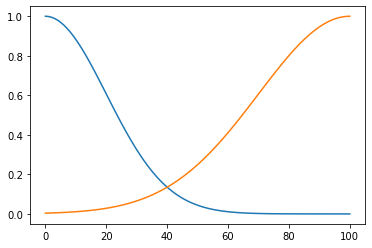
\includegraphics[width=\w\linewidth]{fig/plot03.png}
\caption{Curvas de pertinência, em azul $\mu_{young}$ e em laranja $\mu_{old}$}
\label{fig:plot03}
\end{figure}

\hfill
\section{}  %num4

\par As curvas de pertinências são como na Figura \ref{fig:plot04}.

\[\mu_{a}(x) = \neg \mu_{young}^2 \wedge \neg \mu_{old}^2\]
\[\mu_{b}(x) = \mu_{young}^2 \wedge \mu_{old}^2\]

\begin{figure}[htbp]
\centering
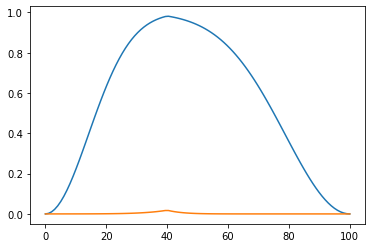
\includegraphics[width=\w\linewidth]{fig/plot04.png}
\caption{Curvas de pertinência, em azul $\mu_{a}$ e em laranja $\mu_{b}$}
\label{fig:plot04}
\end{figure}

\hfill
\section{}  %num5

\[
A_1 = 
\begin{vmatrix}
0.2 & 0.4 & 0.5 \\
\end{vmatrix}
\]

\[
A_2 = 
\begin{vmatrix}
1 & 1 & 0.3 \\
\end{vmatrix}
\]

\[
B_1 = 
\begin{vmatrix}
0.1 & 0.3 \\
\end{vmatrix}
\]

\[
B_1 = 
\begin{vmatrix}
0.6 & 0.2 \\
\end{vmatrix}
\]

\[A_1 \rightarrow B_1\]
\[A_2 \rightarrow B_2\]

\[
A' = 
\begin{vmatrix}
0 & 1 & 0 \\
\end{vmatrix}
\]

\hfill

\[
B' = A' \circ (\underset{i}{\cup} A_i \rightarrow B_i) =
\begin{vmatrix}
b_1 & b_2 \\
\end{vmatrix}
\]

\hfill
\section{}  %num6

\par A curva de pertinência é como na Figura \ref{fig:plot06}.

\[
\mu_{A_1} = trapmf(x, 
\begin{bmatrix}
3 & 4 & 5 & 6 \\
\end{bmatrix})
\]

\[
\mu_{A_2} = trapmf(x, 
\begin{bmatrix}
6 & 6.5 & 7 & 7.5 \\
\end{bmatrix})
\]

\[
\mu_{C_1} = trimf(x, 
\begin{bmatrix}
3 & 4 & 5 \\
\end{bmatrix})
\]

\[
\mu_{C_2} = trimf(x, 
\begin{bmatrix}
4 & 5 & 6 \\
\end{bmatrix})
\]

\[A_1 \rightarrow C_1\]
\[A_2 \rightarrow C_2\]

\[
\mu_{A'} = trimf(x, 
\begin{bmatrix}
5 & 6 & 7 \\
\end{bmatrix})
\]

\hfill

%mt confuso?
\[
\mu_{C'} = \underset{i}{\vee} [\vee (\mu_{A'} \wedge \mu_{A_i}) \wedge \mu_{C_i}]
\]

\begin{figure}[t!]
\centering
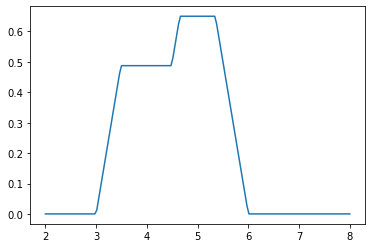
\includegraphics[width=\w\linewidth]{fig/plot06.png}
\caption{Curvas de pertinência de $C'$.}
\label{fig:plot06}
\end{figure}

\end{document}